\documentclass[10pt]{beamer}

\usetheme[progressbar=frametitle]{metropolis}
\usepackage{appendixnumberbeamer}
\usepackage{pgfgantt}
\usepackage{xcolor}
\usepackage{float}
\usepackage{booktabs}
\usepackage[scale=2]{ccicons}
\usepackage{animate}
\usepackage{pgfplots}
\usepgfplotslibrary{dateplot}

\usepackage{xspace}
\newcommand{\themename}{\textbf{\textsc{metropolis}}\xspace}

\title{Exploration of the Changing Nature of Terrorist Attacks}
\subtitle{Using the Global Terrorism Database}
% \date{\today}
\date{}
\author{Jimmy Yue, Taleni Patterson,  Tina Yutong Cao, Matt  Xu Yang, Weihao Xia and  Zoey Zhu}
\institute{University of Sydney}
\titlegraphic{\hfill
\includegraphics[height=1.2cm]{logo.png}}

\begin{document}

\maketitle

%\begin{frame}{Table of contents}
 % \setbeamertemplate{section in toc}[sections numbered]
 % \tableofcontents[hideallsubsections]
%\end{frame}

%\section{Introduction}

\begin{frame}{Motivations and Overview}
    \begin{columns}[T,onlytextwidth]
    \column{0.5\textwidth}
     \begin{block}{What is Terrorism?}
     \begin{itemize}
         \item Acts of violence that incite fear and panic within the public for political, religious or social purposes.
     \end{itemize}
         
     \end{block}
     \column{0.5\textwidth}
    \begin{block}{Changing Awareness}
        \begin{itemize}
            \item After September "9/11" attacks, media coverage and awareness to Terrorist Activity is heightened.
            \item This leads to "A war on Terror" announced by many nations
        \end{itemize}
    \end{block}
     \end{columns}
\end{frame}
%\begin{frame}{Motivations and Overview (ctd.)}
%\begin{columns}[T,onlytextwidth]
 %   \column{0.5\textwidth}
  %  \begin{block}{Changing Awareness}
   %     \begin{itemize}
    %        \item After September "9/11" attacks, media coverage and awareness to Terrorist Activity is heightened.
     %       \item This leads to "A war on Terror" announced by many nations
      %  \end{itemize}
    %\end{block}
    %\column{0.5\textwidth}
    %\begin{figure}[h!]
    %\centering
    %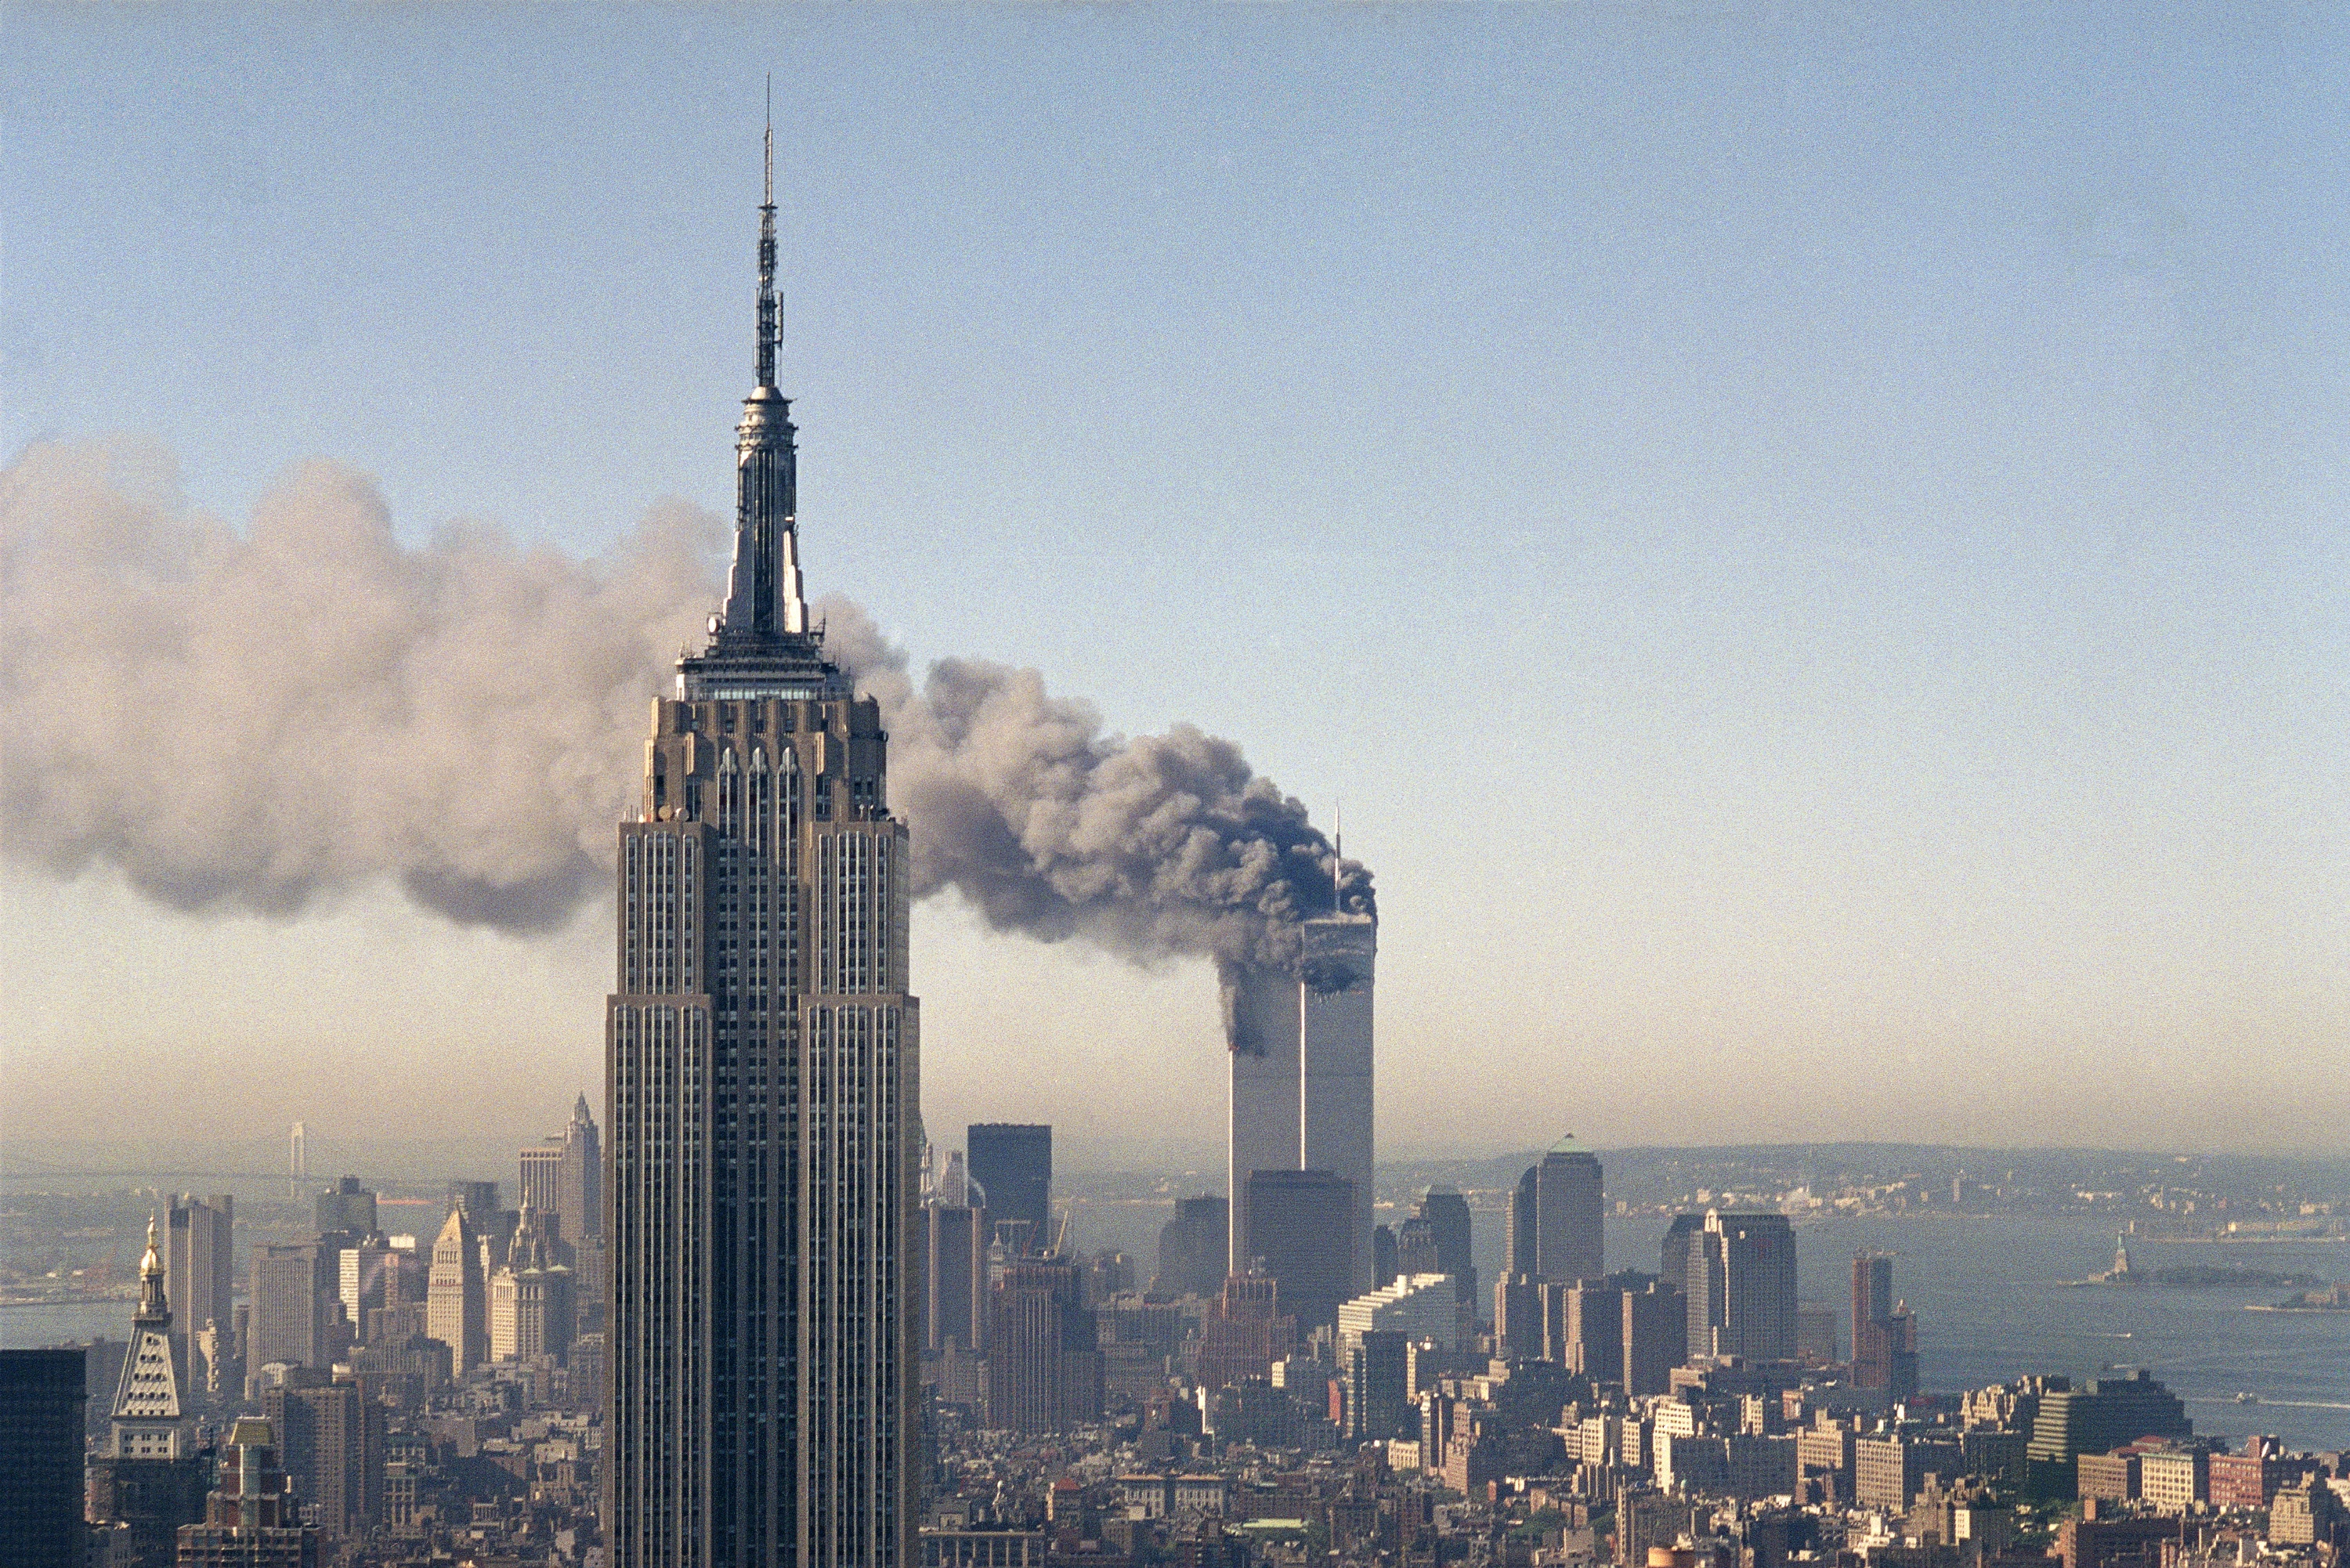
\includegraphics[width= 0.8\textwidth]{20130912000786948627-original.jpg}
    %\caption{September "9/11" attack, \cite{9/11}}
    %\end{figure}
    %\end{columns}
%\end{frame}


%\begin{frame}{Aim}
 %   \begin{alertblock}{Aim}
  %      \begin{itemize}
   %         \item Seek to examine the changing nature of Terrorist Activity with respect to time.
    %    \end{itemize}
    %\end{alertblock}
%\end{frame}


%%%%%%%%%%%%%%%%%%%%DATASET

\begin{frame}{Dataset}
    \begin{block}{The Global Terrorism Database \cite{DataBase}}
        \begin{itemize}
            \item Compiled from multiple non-classified sources \cite{COOKBOOK} such as:
                \begin{itemize}
                    \item [$\diamond$] Media Articles
                    \item [$\diamond$] Legal Documents
                \end{itemize}
            \item The database consists of $181691$ rows and $135$ columns. 
            \item Columns correspond to multiple attributes such as: 
                \begin{itemize}
                    \item [$\diamond$] Number Killed 
                    \item [$\diamond$] Longtitude and Latitude 
                \end{itemize}
            \item Pre-processed and cleaned using \textit{pandas} package.    
        \end{itemize}
    \end{block}
    \begin{exampleblock}{Pre-Processing}
        \begin{itemize}
            \item Correlations between columns and Centrality Measures such as means were examined.
        \end{itemize}
    \end{exampleblock}
\end{frame}

\begin{frame}{Aim \& Tasks}

\begin{alertblock}{Aim}
        \begin{itemize}
            \item Seek to examine the changing nature of Terrorist Activity with respect to time.
        \end{itemize}
    \end{alertblock}

\begin{block}{Tasks}
    \begin{enumerate}
	\item The change in the scale of terrorist attack through examining the number of human casualties along with,
    \item an assessment on the property damage as a monetary value. 
    \item Geography of attacks coupled with a change in geopolitics, 
    %\par\textcolor{red}{(content uploaded to the current folder)}
    \item The change in the differing types of attacks, and what sort of weapons are employed in differing attacks 
    \item along with the types of targets that are targeted.
\end{enumerate}
\end{block}

\end{frame}



%\section{Design and Approaches}

\begin{frame}{Analysis}
   \begin{block}{Design and approach}
       \begin{itemize}
           \item Tableau
           \item Python seaborn and D3
           \item R
       \end{itemize}
   \end{block} 
\end{frame}


\begin{frame}{Visualizations and Implementation}
    \begin{figure}
        \centering
        \includegraphics{}
        \caption{Caption}
        \label{fig:my_label}
    \end{figure}
\end{frame}
\begin{frame}{Visualizations and Implementation (ctd.) }
    
\end{frame}
\begin{frame}{Visualizations and Implementation (ctd.) }
    
\end{frame}



%\subsection{Human Casualties}
%\begin{frame}{Human Casualties}
 %   \begin{alertblock}{What is a Casualty?}
  %  \begin{itemize}
   %     \item We define the class of Casualties as the set union between the number of people killed and the number of people wounded.
    %\end{itemize}
    %\end{alertblock}
   % \begin{block}{Why look at Casualties?}
     %   \begin{itemize}
       %     \item Observing the number of casualties within an incident is indicative of the scale of an attack.
      %  \end{itemize}
   % \end{block}
    %\begin{block}{How can we make visualizations that show a change over time?}
       % \begin{itemize}
           % \item Histograms and Line Graphs are particularly insightful to show if there are specific statistically significant trends that occur.
           % \item Aggregate Geographic Heat-map Visualizations can be used to show the change in geocentrality and severity of human casualties over time.
       % \end{itemize}
    %\end{block}
%\end{frame}
%\subsection{Property Damage}
%\begin{frame}{Property Damage}
%    \begin{alertblock}{How do we measure Property Damage?}
%        \begin{itemize}
%            \item Property damage is measured by looking at the estimated loss of property within an incident in monetary value (USD).
%        \end{itemize}
%    \end{alertblock}
%    \begin{block}{Why look at Property Damage?}
%    \begin{itemize}
%        \item Like human casualties, Property Damage is a variable that can be used to assess the scale of an attack.
%    \end{itemize}
%    \end{block}
%    \begin{block}{How can we make meaningful visualizations that display temporal trends?}
%        \begin{itemize}
%            \item Once again line graphs and histograms can be used to show change over time.
%            \item Similarly to casualties, a heat-map can once again be considered to highlight severity over time.
%        \end{itemize}
%    \end{block}
%\end{frame}
%\subsection{Geography and Geopolitics}

%\begin{frame}{Geography and Geopolitics}
%    \begin{block}{Why is the geographical location of incidents significant?}
%        \begin{itemize}
%            \item INSERT
%        \end{itemize}
%    \end{block}
%    \begin{block}{How can we show the change in location?}
%    \end{block}
%\end{frame}

%\subsection{Types of Attacks}
%\begin{frame}{Types of Attacks}
    
%\end{frame}
%\subsection{Targets}
%\begin{frame}{Targets}
    
%\end{frame}
%\subsection{Holistic Examination}
%\begin{frame}{Holistic Examination}
    
%\end{frame}
%\section{Implementation}

%\section{Evaluation}

\begin{frame}{Evaluation}
    \begin{block}{Comparison with Literature and Similar Studies}
        To assess and evaluate the quality of our visualizations we compared to differing sources such as START and similar Kaggle kernels.
    \end{block}
    \begin{figure}[H]
    \centering
    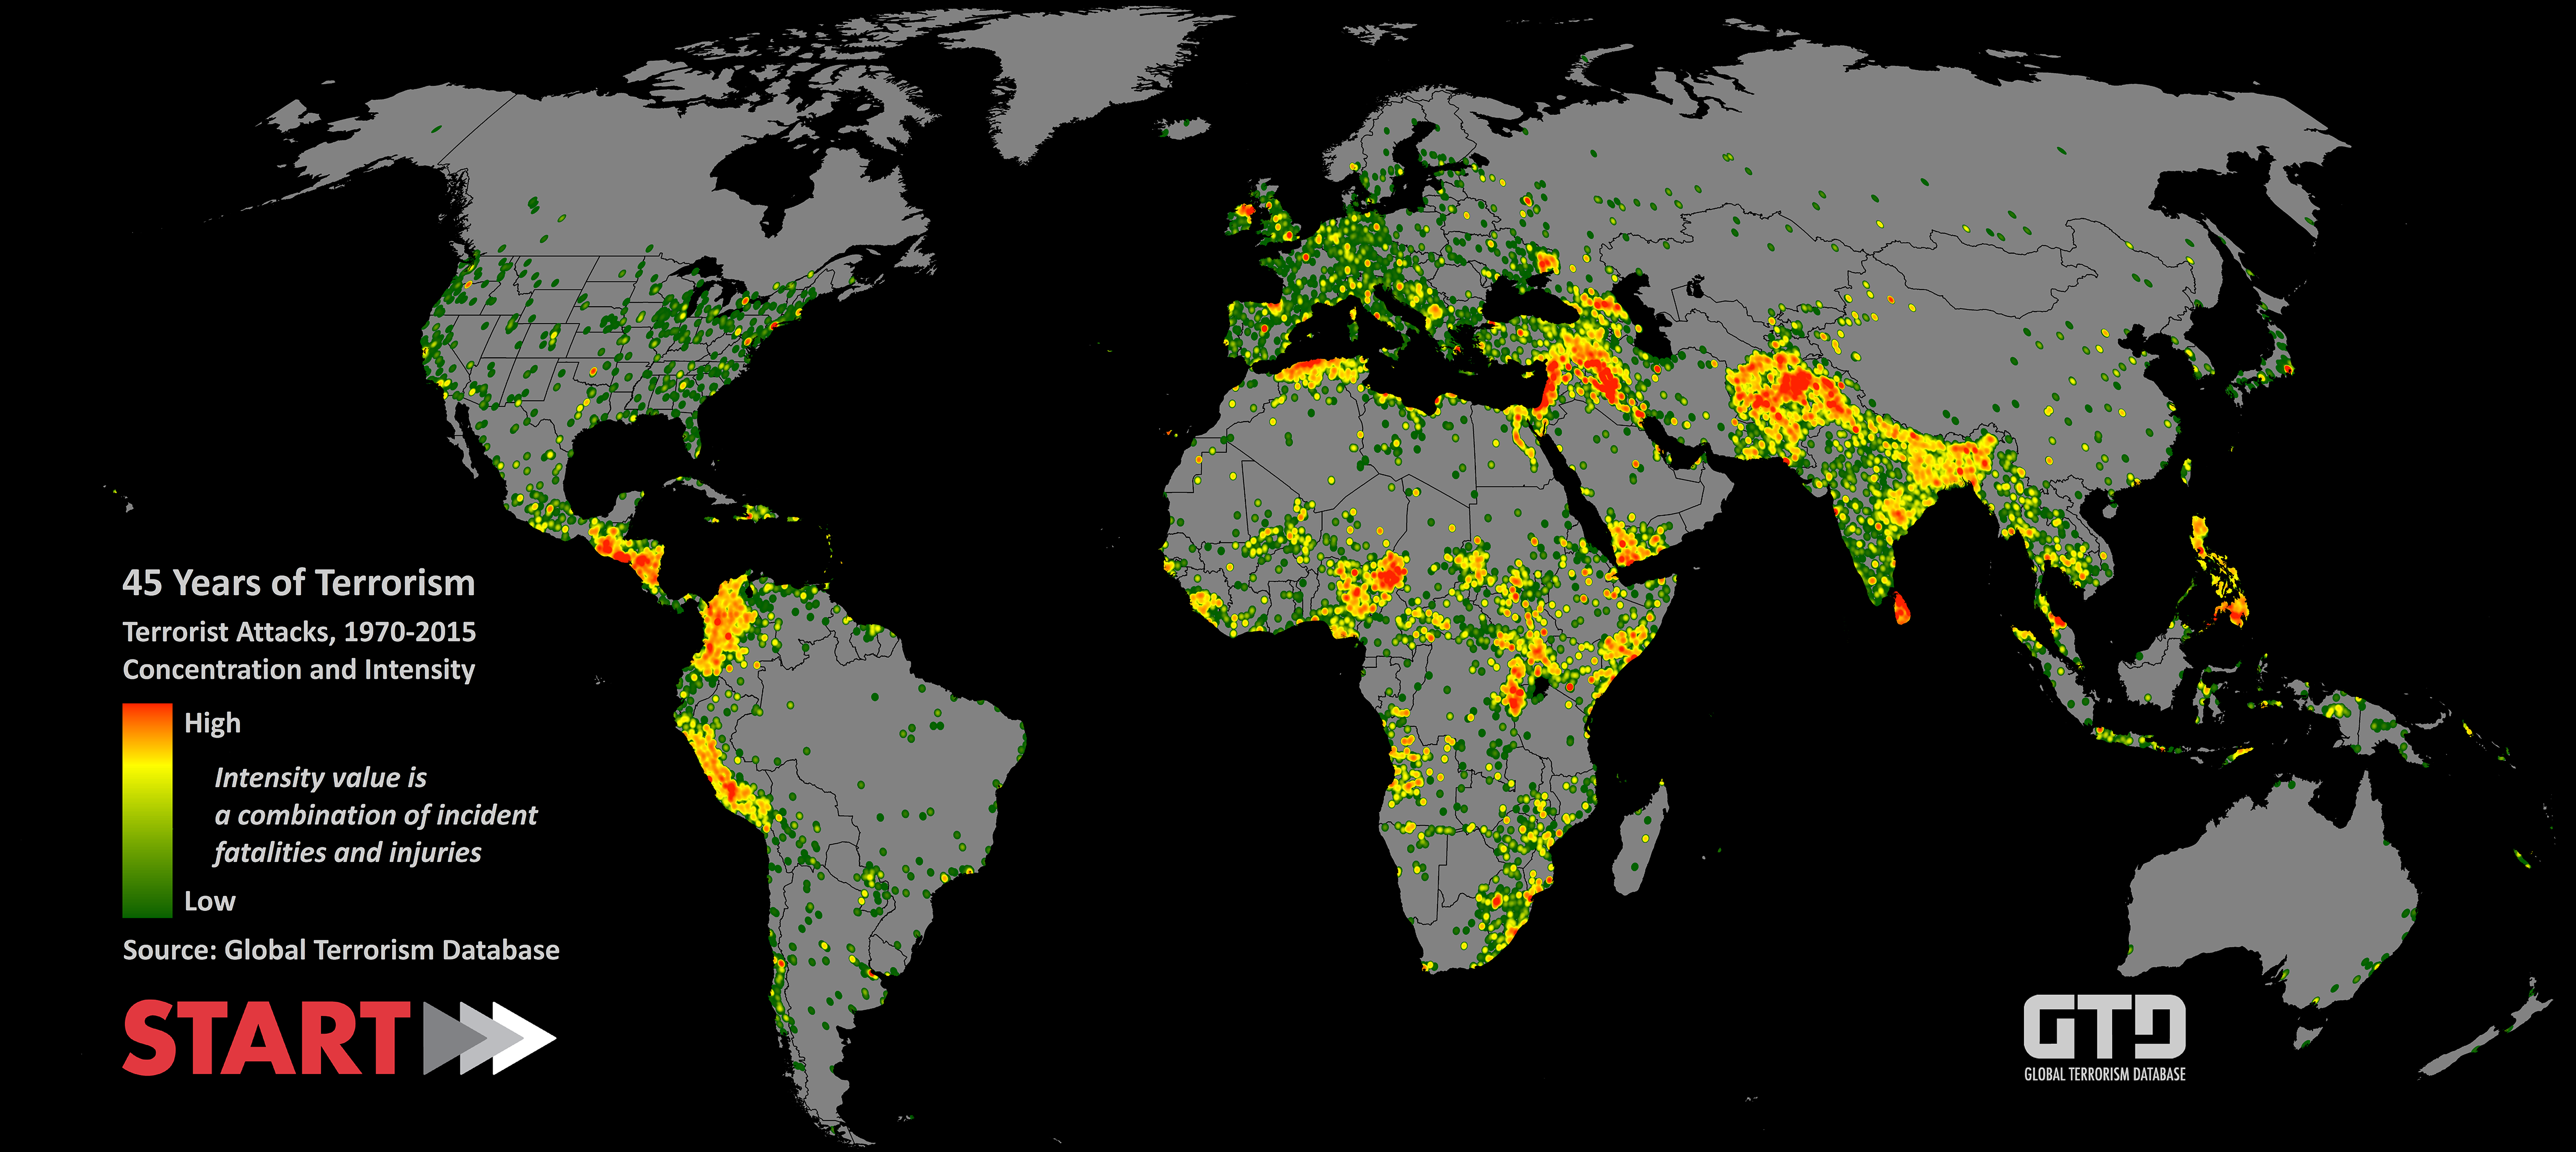
\includegraphics[scale = 0.03]{START_GlobalTerrorismDatabase_TerroristAttacksConcentrationIntensityMap_45Years.png}
    \caption{START Heatmap } 
    \end{figure}
    \begin{block}{Survey}
        \begin{itemize}
            \item A survey will be provided  towards colleagues at workplaces and on social media for visualisation evaluation
        \end{itemize}
    \end{block}
\end{frame}

%\section{Progress and Planning}

\begin{frame}[fragile]{Progress and Planning}
    \definecolor{barblue}{RGB}{153,204,254}
\definecolor{groupblue}{RGB}{51,102,254}
\definecolor{linkred}{RGB}{165,0,33}
\renewcommand\sfdefault{phv}
\renewcommand\mddefault{mc}
\renewcommand\bfdefault{bc}
\setganttlinklabel{s-s}{START-TO-START}
\setganttlinklabel{f-s}{FINISH-TO-START}
\setganttlinklabel{f-f}{FINISH-TO-FINISH}
\sffamily
%\begin{figure}[H]
\centering
\resizebox{0.8\textwidth}{!}{\begin{ganttchart}[
    canvas/.append style={fill=none, draw=black!5, line width=.75pt},
    hgrid style/.style={draw=black!5, line width=.75pt},
    vgrid={*1{draw=black!5, line width=.75pt}},
    today=10,
    today rule/.style={
      draw=black!64,
      dash pattern=on 3.5pt off 4.5pt,
      line width=1.5pt
    },
    today label font=\small\bfseries,
    title/.style={draw=none, fill=none},
    title label font=\bfseries\footnotesize,
    title label node/.append style={below=7pt},
    include title in canvas=false,
    bar label font=\mdseries\small\color{black!70},
    bar label node/.append style={left=2cm},
    bar/.append style={draw=none, fill=black!63},
    bar incomplete/.append style={fill=barblue},
    bar progress label font=\mdseries\footnotesize\color{black!70},
    group incomplete/.append style={fill=groupblue},
    group left shift=0,
    group right shift=0,
    group height=.5,
    group peaks tip position=0,
    group label node/.append style={left=.6cm},
    group progress label font=\bfseries\small,
    link/.style={-latex, line width=1.5pt, linkred},
    link label font=\scriptsize\bfseries,
    link label node/.append style={below left=-2pt and 0pt}
  ]{1}{13}
  \gantttitle[
    title label node/.append style={below left=7pt and -3pt}
  ]{WEEKS:\quad6}{6}
  \gantttitlelist{7,...,13}{1} \\
  \ganttgroup[progress=100]{Preliminary Analysis}{6}{9} \\
  \ganttbar[
    progress=100,
    name=WBS1A
  ]{\textbf{Tableau Exploration} }{6}{9} \\
  \ganttbar[
    progress=100,
    name=WBS1B
  ]{\textbf{Python Exploration} }{6}{9} \\
  \ganttbar[
    progress=100,
    name=WBS1C
  ]{\textbf{R Exploration} }{6}{9} \\
  %\ganttbar[
   % progress=0,
    %name=WBS1D
  %]{\textbf{WBS 1.4} Activity D}{4}{10} \\[grid]
  \ganttgroup[progress=0]{Data Analysis and Plot Generation Split between group members}{8}{12} \\
  \ganttbar[progress=80]{\textbf{Casualty Plots}}{8}{11} \\
  \ganttbar[progress=80]{\textbf{Property Damage Plots}}{8}{11} \\
  \ganttbar[progress=60]{\textbf{Geovisualisations}}{8}{11} \\
  \ganttbar[progress=80]{\textbf{Weapons types}}{8}{11} \\
  \ganttbar[progress=80]{\textbf{Types of Attacks}}{8}{11}\\
   \ganttbar[progress=50]{\textbf{Casualty compared to others}}{9}{12}\\
    \ganttbar[progress=50]{\textbf{Property Damage compared to others}}{9}{12}\\
     \ganttbar[progress=30]{\textbf{Geographical plots compared to others}}{9}{12}\\
      \ganttbar[progress=50]{\textbf{Weapon types compared to others}}{9}{12}\\
       \ganttbar[progress=50]{\textbf{Attack types compared to others}}{9}{12}\\
  \ganttgroup[progress=60]{Report Writing and Analysis of Plots}{7}{12} \\
  
\end{ganttchart}}
%\caption{Gant chart of planned work progress in the project}
%\end{figure}
\end{frame}


%\begin{frame}[fragile]{Metropolis}

 % The \themename theme is a Beamer theme with minimal visual noise
  %inspired by the \href{https://github.com/hsrmbeamertheme/hsrmbeamertheme}{\textsc{hsrm} Beamer
  %Theme} by Benjamin Weiss.

  %Enable the theme by loading

 % \begin{verbatim}    \documentclass{beamer}
  %  \usetheme{metropolis}\end{verbatim}

  %Note, that you have to have Mozilla's \emph{Fira Sans} font and XeTeX
  %installed to enjoy this wonderful typography.
%\end{frame}
%\begin{frame}[fragile]{Sections}
 % Sections group slides of the same topic

  %\begin{verbatim}    \section{Elements}\end{verbatim}

  %for which \themename provides a nice progress indicator \ldots
%\end{frame}

%\section{Titleformats}

%\begin{frame}{Metropolis titleformats}
%	\themename supports 4 different titleformats:
%	\begin{itemize}
%		\item Regular
%		\item \textsc{Smallcaps}
%		\item \textsc{allsmallcaps}
%		\item ALLCAPS
%	\end{itemize}
%	They can either be set at once for every title type or individually.
%\end{frame}

%{
 %   \metroset{titleformat frame=smallcaps}
%\begin{frame}{Small caps}
%	This frame uses the \texttt{smallcaps} titleformat.

%	\begin{alertblock}{Potential Problems}
%		Be aware, that not every font supports small caps. If for example you typeset your presentation with pdfTeX and the Computer Modern Sans Serif font, every text in smallcaps will be typeset with the Computer Modern Serif font instead.
%	\end{alertblock}
%\end{frame}
%}

%{
%\metroset{titleformat frame=allsmallcaps}
%\begin{frame}{All small caps}
%	This frame uses the \texttt{allsmallcaps} titleformat.

%	\begin{alertblock}{Potential problems}
%		As this titleformat also uses smallcaps you face the same problems as with the \texttt{smallcaps} titleformat. Additionally this format can cause some other problems. Please refer to the documentation if you consider using it.

%		As a rule of thumb: Just use it for plaintext-only titles.
%	\end{alertblock}
%\end{frame}
%}

%{
%\metroset{titleformat frame=allcaps}
%\begin{frame}{All caps}
%	This frame uses the \texttt{allcaps} titleformat.

%	\begin{alertblock}{Potential Problems}
%		This titleformat is not as problematic as the \texttt{allsmallcaps} format, but basically suffers from the same deficiencies. So please have a look at the documentation if you want to use it.
%	\end{alertblock}
%\end{frame}
%}

%\section{Elements}

%\begin{frame}[fragile]{Typography}
 %     \begin{verbatim}The theme provides sensible defaults to
%\emph{emphasize} text, \alert{accent} parts
%or show \textbf{bold} results.\end{verbatim}

 % \begin{center}becomes\end{center}

  %The theme provides sensible defaults to \emph{emphasize} text,
  %\alert{accent} parts or show \textbf{bold} results.
%\end{frame}

%\begin{frame}{Font feature test}
 % \begin{itemize}
  %  \item Regular
   % \item \textit{Italic}
    %\item \textsc{SmallCaps}
    %\item \textbf{Bold}
    %\item \textbf{\textit{Bold Italic}}
    %\item \textbf{\textsc{Bold SmallCaps}}
    %\item \texttt{Monospace}
    %\item \texttt{\textit{Monospace Italic}}
    %\item \texttt{\textbf{Monospace Bold}}
    %item \texttt{\textbf{\textit{Monospace Bold Italic}}}
  %\end{itemize}
%\end{frame}

%\begin{frame}{Lists}
 % \begin{columns}[T,onlytextwidth]
  %  \column{0.33\textwidth}
   %   Items
    %  \begin{itemize}
     %   \item Milk \item Eggs \item Potatos
     % \end{itemize}

    %\column{0.33\textwidth}
     % Enumerations
      %\begin{enumerate}
       % \item First, \item Second and \item Last.
      %\end{enumerate}

    %\column{0.33\textwidth}
     % Descriptions
      %\begin{description}
       % \item[PowerPoint] Meeh. \item[Beamer] Yeeeha.
      %\end{description}
  %\end{columns}
%\end{frame}
%\begin{frame}{Animation}
 % \begin{itemize}[<+- | alert@+>]
  %  \item \alert<4>{This is\only<4>{ really} important}
   % \item Now this
    %\item And now this
  %\end{itemize}
%\end{frame}
%\begin{frame}{Figures}
 % \begin{figure}
  %  \newcounter{density}
   % \setcounter{density}{20}
    %\begin{tikzpicture}
     % \def\couleur{alerted text.fg}
      %\path[coordinate] (0,0)  coordinate(A)
      %            ++( 90:5cm) coordinate(B)
       %           ++(0:5cm) coordinate(C)
        %          ++(-90:5cm) coordinate(D);
      %\draw[fill=\couleur!\thedensity] (A) -- (B) -- (C) --(D) -- cycle;
      %\foreach \x in {1,...,40}{%
          %\pgfmathsetcounter{density}{\thedensity+20}
          %\setcounter{density}{\thedensity}
          %\path[coordinate] coordinate(X) at (A){};
          %\path[coordinate] (A) -- (B) coordinate[pos=.10](A)
                              -- %(C) coordinate[pos=.10](B)
                              -- %(D) coordinate[pos=.10](C)
                              -- %(X) coordinate[pos=.10](D);
          %\draw[fill=\couleur!\thedensity] (A)--(B)--(C)-- (D) -- cycle;
      %}
    %\end{tikzpicture}
    %\caption{Rotated square from
    %\href{http://www.texample.net/tikz/examples/rotated-polygons/}{texample.net}.}
  %\end{figure}
%\end{frame}
%\begin{frame}{Tables}
 % \begin{table}
  %  \caption{Largest cities in the world (source: Wikipedia)}
  %  \begin{tabular}{lr}
   %   \toprule
    %  City & Population\\
     % \midrule
      %Mexico City & 20,116,842\\
      %Shanghai & 19,210,000\\
      %Peking & 15,796,450\\
      %Istanbul & 14,160,467\\
      %\bottomrule
    %\end{tabular}
  %\end{table}
%\end{frame}
%\begin{frame}{Blocks}
  %Three different block environments are pre-defined and may be styled with an
  %optional background color.

  %\begin{columns}[T,onlytextwidth]
   % \column{0.5\textwidth}
    %  \begin{block}{Default}
     %   Block content.
      %\end{block}

      %\begin{alertblock}{Alert}
       % Block content.
      %\end{alertblock}

      %\begin{exampleblock}{Example}
       % Block content.
      %\end{exampleblock}

    %\column{0.5\textwidth}

     % \metroset{block=fill}

      %\begin{block}{Default}
       % Block content.
      %\end{block}

      %\begin{alertblock}{Alert}
       % Block content.
      %\end{alertblock}

      %\begin{exampleblock}{Example}
       % Block content.
      %\end{exampleblock}

  %\end{columns}
%\end{frame}
%\begin{frame}{Math}
 % \begin{equation*}
  %  e = \lim_{n\to \infty} \left(1 + \frac{1}{n}\right)^n
  %\end{equation*}
%\end{frame}
%\begin{frame}{Line plots}
 % \begin{figure}
  %  \begin{tikzpicture}
   %   \begin{axis}[
    %    mlineplot,
     %   width=0.9\textwidth,
      %  height=6cm,
      %]

       % \addplot {sin(deg(x))};
        %\addplot+[samples=100] {sin(deg(2*x))};

      %\end{axis}
    %\end{tikzpicture}
  %\end{figure}
%\end{frame}
%\begin{frame}{Bar charts}
 % \begin{figure}
  %  \begin{tikzpicture}
   %   \begin{axis}[
    %    mbarplot,
     %   xlabel={Foo},
      %  ylabel={Bar},
        %width=0.9\textwidth,
       % height=6cm,
      %]

      %\addplot plot coordinates {(1, 20) (2, 25) (3, 22.4) (4, 12.4)};
      %\addplot plot coordinates {(1, 18) (2, 24) (3, 23.5) (4, 13.2)};
      %\addplot plot coordinates {(1, 10) (2, 19) (3, 25) (4, 15.2)};

      %\legend{lorem, ipsum, dolor}

      %\end{axis}
    %\end{tikzpicture}
  %\end{figure}
%\end{frame}
%\begin{frame}{Quotes}
 % \begin{quote}
  %  Veni, Vidi, Vici
  %\end{quote}
%\end{frame}

%{%
%\setbeamertemplate{frame footer}{My custom footer}
%\begin{frame}[fragile]{Frame footer}
%    \themename defines a custom beamer template to add a text to the footer. It can be set via
%    \begin{verbatim}\setbeamertemplate{frame footer}{My custom footer}\end{verbatim}
%\end{frame}
%}

%\begin{frame}{References}
 % Some references to showcase [allowframebreaks] \cite{knuth92,ConcreteMath,Simpson,Er01,greenwade93}
%\end{frame}

%\section{Conclusion}

%\begin{frame}{Summary}

 % Get the source of this theme and the demo presentation from

  %\begin{center}\url{github.com/matze/mtheme}\end{center}

  %The theme \emph{itself} is licensed under a
  %\href{http://creativecommons.org/licenses/by-sa/4.0/}{Creative Commons
  %Attribution-ShareAlike 4.0 International License}.

  %\begin{center}\ccbysa\end{center}

%\end{frame}

%{\setbeamercolor{palette primary}{fg=black, bg=yellow}
%\begin{frame}[standout]
%  Questions?
%\end{frame}
%}
%
%\appendix

%\begin{frame}[fragile]{Backup slides}
 % Sometimes, it is useful to add slides at the end of your presentation to
 % refer to during audience questions.

  %The best way to do this is to include the \verb|appendixnumberbeamer|
  %package in your preamble and call \verb|\appendix| before your backup slides.

  %\themename will automatically turn off slide numbering and progress bars for
  %slides in the appendix.
%\end{frame}

\begin{frame}[allowframebreaks]{References}

 \bibliography{demo}
  \bibliographystyle{unsrt}

\end{frame}

\end{document}
